\documentclass{scrartcl}

\usepackage[utf8]{inputenc}
\usepackage[T1]{fontenc}
\usepackage[francais]{babel}
\usepackage{amsmath}
\usepackage{amsfonts}
\usepackage{geometry}
\usepackage{graphicx}
\usepackage{url}
\usepackage{amsthm}
\usepackage{float}
%\usepackage{mathpazo}

%\usepackage{newpx}
\geometry{hmargin=2.5cm,vmargin=2cm}

\DeclareMathOperator*{\argmax}{\arg\!\max}
\newtheorem*{Prob}{Problème}
\newtheorem*{lemma}{Lemme}
\newtheorem*{hypo}{Hypothèse}
\newtheorem*{defi}{Définition}

\title{Rapport de stage de L3}
\subtitle{Cryptanalyse linéaire expérimentale de DES}
\author{Lucas Pesenti}
\date{juin -- juillet 2017}

\begin{document}
\maketitle
\tableofcontents
\newpage

\section{Introduction}
\paragraph*{}
Historiquement, les techniques de cryptanalyse linéaire ont été mises en pratique pour la première fois
par Matsui dans \cite{Matsui1994}. À l'époque de la publication, la cible privilégiée de ce type
d'attaque était alors DES, le principal algorithme de chiffrement symétrique en vigueur. Même si celui-ci
n'est aujourd'hui normalement quasiment plus utilisé sous sa forme originelle, au profit notamment d'AES,
il reste un objet d'étude intéressant pour la cryptographie expérimentale.

Il s'agit d'une attaque à clair connu : on détermine certains bits de la clé à partir d'approximations
linéaires biaisées entre l'entrée et la sortie de l'algorithme et d'un certain nombre de couples
clair/chiffré. Ensuite, il ne reste plus qu'à essayer exhaustivement toutes les combinaisons de bits restantes. La position
de la bonne clé dans ce parcours est appelé son \textit{rang}, et l'objectif de toute méthode de cryptanalyse
linéaire est de minimiser cette quantité.

Néanmoins, en pratique, les meilleures attaques connues sur DES reposent toujours sur un parcours
exhaustif de l'espace des clés (voir par exemple \cite{crack}). En effet, toutes les attaques linéaires
connues rencontrent un obstacle pratique : la complexité en donnée, à savoir le nombre de couples clair/chiffré
dont on suppose disposer initialement. Par exemple, \cite{Junod2001} montre que l'attaque classique de Matsui
nécessite $2^{43}$ entrées chiffrées avec la bonne clé pour obtenir un rang inférieur à $2^{41}$ (sur
$2^{56}$ clés au total) dans 85\% des cas.

Les travaux plus récents en cryptanalyse linéaire s'attachent principalement à montrer que les
hypothèses d'indépendance faites dans les modèles d'attaque sont inexactes en théorie. À l'inverse, l'aspect
expérimental est souvent mis de côté.

\paragraph*{}
L'objectif de mon stage, réalisé sous la direction de François-Xavier Standaert dans l'équipe
UCL Crypto à Louvain-la-Neuve (Belgique), était en conséquence de proposer une attaque linéaire complète de DES en utilisant
des méthodes pour optimiser chaque étape de la cryptanalyse. J'ai notamment cherché un compromis entre
la complexité en donnée et le rang de la clé.

\paragraph*{}
Plus précisément, mon travail peut être découpé en différentes parties.

\begin{itemize}
	\item \textbf{Génération des approximations linéaires de DES} : l'algorithme de Matsui, présenté dans \cite{Matsui1995}, est à
	ma connaissance le seul outil utilisé dans ce domaine. Je propose de supprimer une hypothèse d'indépendance faite dans
	celui-ci en modifiant la phase de génération des approximations linéaires sur 1 round. L'objectif est de permettre
	une meilleure évaluation des biais à l'issue de cette phase. J'implémente ensuite la méthode de Branch\&Bound de Matsui
	pour en déduire les meilleures approximations sur 14 rounds.
	\item \textbf{Cryptanalyse linéaire multidimensionnelle} : l'objectif de cette attaque est d'exploiter pleinement la donnée de
	plusieurs approximations linéaires portant sur un même ensemble de bits de clé. Deux modèles de cryptanalyse multilinéaire
	existent : celui de Biryukov \cite{Biryukov2004} et celui d'Hermelin \cite{TheseHermelin}. J'ai choisi ce dernier, qui
	est plus transparent sur ses hypothèses d'indépendance.
	\item \textbf{Combinaison de différentes attaques multilinéaires} : j'utilise dans cette optique les nouveaux outils
	d'énumération de clé et d'estimation de rang, décrits dans \cite{ches-2016} et développés dans mon équipe d'accueil dans le cadre
	des attaques side-channel. Cela m'a permis en particulier de tester l'efficacité des méthodes développées en évaluant
	très efficacement le rang de la clé.
\end{itemize}

\paragraph*{}
La majorité du programme de cryptanalyse \cite{github} a été écrit en C++, avec quelques programmes utilitaires en Python. J'utilise  pour
l'estimation de rang le code open-source fourni avec \cite{ches-2016}, qui nécessite lui-même la bibliothèque NTL \cite{ntl}.

\section{Notations}

\paragraph*{}
Dans tout ce qui suit, $k_0$ désigne la clé fixée qu'on cherche à casser et $\text{DES}=\text{DES}_{k_0}$
la fonction DES (voir \textsc{Figure} \ref{deswiki}).

En particulier, l'entrée $u$ et la sortie $v$ d'un certain round peuvent être vus comme des éléments de l'algèbre
$\mathbb{F}_2^{64}$, sur laquelle s'appliquent les opérations usuelles d'addition (induite par $\mathbb{F}_2$)
et de produit scalaire :

$$\forall \alpha, \beta \in \mathbb{F}_2^{64}, \alpha \cdot \beta = \sum_{i=1}^{64} \alpha_i \beta_i$$

\paragraph*{}
On fixe une distribution de probabilité $P$ uniforme sur les entrées. Dans ce cadre formel, une
\textit{approximation linéaire du DES sur $n$ rounds} est un triplet de masques $(\alpha, \beta, \gamma)$ portant
respectivement sur l'entrée $u$ du DES, la sortie $v$ du $n$-ème round et la clé $k_0$. On définit son \textit{biais} $\epsilon$ par :

$$\epsilon=\left|P(\alpha \cdot u + \beta \cdot v=\gamma \cdot k_0)-\frac{1}{2}\right|$$

Dans le cadre de la cryptanalyse multidimensionnelle, on sera amené à travailler avec un système de $m$ approximations $(A,B,\Gamma)$ de
la forme :

$$Au+Bv=\Gamma k_0$$

où $A,B,\Gamma$ sont des matrices $m\times 64$. On réutilise la notion de \textit{capacité} $C$ du système d'approximations, introduite dans
$\cite{TheseHermelin}$ :

$$C=\sum_{\eta=0}^{2^m-1}\left(P(Au+Bv=\eta)-\frac{1}{2^m}\right)^2$$

On peut l'interpréter comme la distance $l^2$ entre la distribution induite par les approximations et la distribution uniforme.\footnote{En fait,
il s'agit plus exactement du premier terme du développement de Taylor de la distance de Kullback-Leibler entre ces deux distributions.}

\paragraph*{}
On rappelle le très utile lemme Piling-Up :

\begin{lemma}[Piling-Up]
	Si $X_1, \ldots X_n$ sont des variables aléatoires indépendantes à valeurs dans $\{0,1\}$, alors :

$$P(X_1 \oplus \ldots \oplus X_n=0)=\frac{1}{2}+2^{n-1}\prod_{i=1}^n \left(P(X_i=0)-\frac{1}{2}\right)$$
\end{lemma}

\paragraph*{}
Enfin, la complexité en donnée sera notée $N$.

\section{Génération des approximations linéaires}

\paragraph*{}
La première étape dans la cryptanalyse de DES consiste à générer des approximations linéaires biaisées. En anticipant sur la phase
suivante, on utilise la formule heuristique $N \approx 1/\epsilon^2$ dérivée initialement par Matsui dans le cadre de la cryptanalyse linéaire
simple. \footnote{En cryptanalyse multilinéaire, on a la formule approchée $N \approx 1/C$.} On cherche donc à maximiser le biais des approximations choisies.

On appellera \textit{approximations de Matsui sur $n$ rounds} les deux approximations de biais maximal du DES restreint à $n$ rounds, explicitées dans l'annexe de \cite{Matsui1994}. Les
approximations de Matsui sur $14$ rounds ont la particularité de porter sur deux ensembles de bits disjoints, phénomène
qu'on utilisera dans la phase d'estimation de rang.

Dans le cadre de mon stage, la volonté de trouver des meilleures approximations que celles connues actuellement était motivée par l'absence supposée
de l'effet de \textit{linear hull} \cite{Nyberg1995} avec DES. En effet, lorsque celui-ci ne se manifeste pas, il existe généralement une paire
de masques d'entrée/sortie sur lesquels portent des approximations biaisées ; pour autant, on ne sait pas exhiber des approximations dominantes pour DES.

\subsection{Déchiffrement partiel}

\paragraph*{}
On se demande tout d'abord sur combien de rounds les approximations doivent porter. En effet, l'algorithme 2 de Matsui, qu'on utilise dans
la phase de cryptanalyse, consiste à deviner une partie des bits de la clé en déchiffrant partiellement l'entrée ou la sortie. Pour cela,
on étudie le nombre de bits de clé dont il faut connaître la valeur pour calculer la sortie de la $j$-ème S-box du $i$-ème round.

Les résultats sont représentés sur la \textsc{Figure} \ref{arraybit}. Ils confirment la bonne diffusion des P-box : le nombre de bits
de dépendance $r$ explose très rapidement. Étant donné qu'on aura besoin d'un facteur temporel $2^r$ pour le traiter, on n'envisage 
le gain que d'un seul round en entrée et en sortie du DES. L'objectif devient dès lors de trouver les meilleures approximations linéaires
du DES restreint à 14 rounds.


\subsection{Algorithme de Matsui de génération des approximations linéaires}

\paragraph*{}
L'algorithme classique de Matsui est décrit dans \cite{Matsui1995} et \cite{Biryukov2004} le reprend sous
une forme quasiment identique. Il fonctionne comme suit :


\begin{itemize}
	\item on visualise chacune des 8 S-box comme une fonction de 6 bits dans 4 bits. On précalcule exhaustivement les
	biais de toutes les approximations linéaires de cette fonction. À ce stade, en supposant que les entrées des
	différentes S-box sont indépendantes, on connaît les biais de toutes les approximations linéaires sur 1 round de DES
	par le lemme Piling-Up ;
	\item on applique une recherche Branch\&Bound pour combiner les approximations d'un round sur 14 rounds.
\end{itemize}

\paragraph*{}
En particulier, pour calculer les biais des approximations finales avec le lemme Piling-Up, les hypothèses implicites suivantes sont faites :

\begin{itemize}
	\item indépendance verticale : les entrées successives des différents rounds de DES sont indépendantes ; 
	\item indépendance horizontale : les entrées des différentes S-box d'un même round sont indépendantes. 
\end{itemize}

\paragraph*{}
On se concentre ici sur la deuxième hypothèse. Comme le montre la \textsc{Figure} \ref{fig:exp}, pour passer de l'entrée de $F$ sur 32 bits aux
48 bits en entrée des S-box, 16 bits sont dupliqués entre deux S-box par la fonction d'expansion. L'application horizontale
du lemme Piling-Up ne paraît donc pas justifiée.

\subsection{Un meilleur algorithme de génération sur 1 round}

\paragraph*{}
J'ai cherché et implémenté un algorithme pour déterminer les meilleures approximations linéaires du DES sur 1 round, en se
passant de l'hypothèse d'indépendance horizontale.

\subsubsection{Réduction à OFF-MIPS}

\paragraph*{}
Considérons le problème OFF-MIPS (pour \textit{OFFline Maximum Inner Product Search}) suivant :

\begin{Prob}[OFF-MIPS]
Soient $(l_i)_{1\le i\le n}$ et $(r_j)_{1\le j\le n}$ deux listes de vecteurs de $\mathbf{R}^d$. On veut trouver
	$$\underset{1\le j\le n}{\underset{1\le i\le n}{\argmax}}\langle l_i,r_j\rangle$$
où $\langle\cdot,\cdot\rangle$ est le produit scalaire canonique sur $\mathbf{R}^d$.
\end{Prob}

En réalité, on aura besoin de résoudre le problème plus général $s$-OFF-MIPS, à savoir récupérer les $s$ paires $(i,j)$ donnant
les $s$ plus grandes valeurs de $\langle l_i,r_j\rangle$.

\paragraph*{}
On va réduire la recherche des $s$ meilleures approximations du DES sur 1 round à $s$-OFF-MIPS.
Considérons une approximation $(\alpha, \beta, \gamma)$ de 32 bits sur 1 round. On veut calculer :
$$p=P(\alpha\cdot u + \beta\cdot v=\gamma\cdot k)$$

où $u$ (resp. $v$) est l'entrée (resp. la sortie) de la fonction $F$ de ce round.

\paragraph*{}
Remarquons que la fonction d'expansion a une forme particulière : chaque S-box partage avec son voisin de gauche
(resp. de droite) exactement deux entrées communes (voir \textsc{Figure} \ref{fig:exp}).

On numérote les entrées $E_1, \ldots, E_{48}$ et les sorties $S_1, \ldots S_{32}$, conformément à la \textsc{Figure} \ref{fig:inout}.



\paragraph*{}
Fixons les valeurs $(b_1, \ldots, b_{16})$ des entrées communes à plusieurs S-box et notons $P'$ la distribution conditionnelle
suivante :

$$P' = P(\cdot | E_1=b_1, E_2=b_2, E_5=b_3, E_6=b_4,\ldots)$$

Relativement à la mesure $P'$, les entrées et les sorties des différentes S-box sont maintenant indépendantes, de sorte qu'on peut appliquer
le lemme Piling-Up. En considérant qu'une entrée correspond toujours à la S-box la plus à droite à laquelle elle est reliée, 
on note $\alpha^{(i)}$ (resp. $\beta^{(i)}$) le masque $\alpha$ (resp. $\beta$) restreint aux entrées (resp. sorties)
de la $i$-ème S-box. Alors :

\begin{align*}
	P'(\alpha\cdot u+\beta\cdot v=\gamma\cdot k)&=\frac{1}{2}+2^{7}\prod_{i=1}^8 \left(P'(\alpha^{(i)}\cdot u+\beta^{(i)}\cdot v =\gamma\cdot k)-\frac{1}{2}\right)\\
\end{align*}

Donc, en notant :

$$M^{(1)}_{b_1,b_2,b_3,b_4}=P(\alpha^{(1)}\cdot u+\beta^{(1)}\cdot v=\gamma\cdot k|E_1=b_1,E_2=b_2,E_5=b_3,E_6=b_6)-\frac{1}{2}$$

on a :

\begin{align*}
	p=\frac{1}{2}+\frac{2^7}{2^4} \sum_{b_1, b_2,b_3,b_4\in \{0,1\}} M^{(1)}_{b_1,b_2,b_3,b_4} \prod_{i=2}^8 \left(P'(\alpha^{(i)}\cdot u+\beta^{(i)}\cdot v =\gamma\cdot k)-\frac{1}{2}\right)
\end{align*}

De même, avec :

$$M^{(2)}_{b_3,b_4,b_5,b_6}=P(\alpha^{(2)}\cdot u+\beta^{(2)}\cdot v=\gamma\cdot k|E_7=b_3,E_8=b_4,E_{11}=b_5,E_{12}=b_6)-\frac{1}{2}$$

on obtient :

\begin{align*}
	p=\frac{1}{2}+\frac{2^7}{2^6} \sum_{b_1,\ldots, b_6\in \{0,1\}} M^{(1)}_{b_1,b_2,b_3,b_4} M^{(2)}_{b_3,b_4,b_5,b_6} \prod_{i=3}^8 \left(P'(\alpha^{(i)}\cdot u+\beta^{(i)}\cdot v =\gamma\cdot k)-\frac{1}{2}\right)
\end{align*}

Ainsi, par récurrence, on définit :

$$M^{(i)}_{b_{2i-1},b_{2i},b_{2i+1},b_{2i+2}}=P(\alpha^{(i)}\cdot u+\beta^{(i)}\cdot v=\gamma\cdot k|(E_{6i-5},E_{6i-4},E_{6i-1},E_{6i})=(b_{2i-1},\ldots,b_{2i+2}))-\frac{1}{2}$$

d'où :

\begin{align*}
	p=\frac{1}{2}+\frac{2^7}{2^{16}} \sum_{b_1,\ldots, b_{16}\in \{0,1\}} M^{(1)}_{b_1,b_2,b_3,b_4} M^{(2)}_{b_3,b_4,b_5,b_6}\ldots M^{(7)}_{b_{13},b_{14},b_{15},b_{16}} M^{(8)}_{b_{15},b_{16},b_1,b_2}
\end{align*}

\paragraph*{}
On interprète la formule comme un produit matriciel en posant :

$$M^{(i)}=\begin{bmatrix}
	M^{(i)}_{0,0,0,0} & M^{(i)}_{0,0,0,1} & M^{(i)}_{0,0,1,0} & M^{(i)}_{0,0,1,1}\\
	M^{(i)}_{0,1,0,0} & M^{(i)}_{0,1,0,1} & M^{(i)}_{0,1,1,0} & M^{(i)}_{0,1,1,1}\\
	M^{(i)}_{1,0,0,0} & M^{(i)}_{1,0,0,1} & M^{(i)}_{1,0,1,0} & M^{(i)}_{1,0,1,1}\\
	M^{(i)}_{1,1,0,0} & M^{(i)}_{1,1,0,1} & M^{(i)}_{1,1,1,0} & M^{(i)}_{1,1,1,1}
\end{bmatrix}$$

Dans ce contexte, avec $\text{Tr}$ l'application trace : 

$$p=\frac{1}{2}+\frac{1}{2^9} \text{Tr}(M^{(1)}\ldots M^{(8)})$$

\paragraph*{}
Finalement, on sait que le produit scalaire défini par :

$$\forall A,B\in \mathcal{M}_{4,4}(\mathbf{R}), \langle A,B\rangle=\text{Tr}(A^T B)$$

correspond exactement au produit scalaire canonique de $\mathbf{R}^{16}$.

\paragraph*{}
Ainsi, pour se ramener à OFF-MIPS, on calcule dans un premier temps l'ensemble $\mathcal{A}^{(i)}$ des matrices $M^{(i)}$
en faisant varier $\alpha^{(i)}$ et $\beta^{(i)}$ grâce au précalcul des biais des approximations linéaires d'une S-box.
Le cardinal de chaque $\mathcal{A}^{(i)}$ est $2^8=256$. Dans un second temps,
on génère les ensembles :

$$\mathcal{L}=\{(M^{(1)}\ldots M^{(4)})^T, (M^{(1)}, \ldots M^{(4)})\in \mathcal{A}^{(1)}\times \ldots \times \mathcal{A}^{(4)}\}$$

et :
$$\mathcal{R}=\{M^{(5)}\ldots M^{(8)}, (M^{(5)}, \ldots M^{(8)})\in \mathcal{A}^{(5)}\times \ldots \times \mathcal{A}^{(8)}\}$$

Finalement, le meilleur biais d'une approximation d'un round de DES s'exprime comme :

$$\epsilon=\frac{1}{2^9}\underset{R\in\mathcal{R}}{\underset{L\in\mathcal{L}}{\max}}|\langle L,R\rangle|$$

où chaque matrice de $\mathcal{L}$ et $\mathcal{R}$ est interprétée comme un vecteur de $\mathbf{R}^{16}$. Ceci conclut la réduction vers
OFF-MIPS.

\subsubsection{Détails d'implémentation}

Les ensembles $\mathcal{L}$ et $\mathcal{R}$ étant de taille $2^{32}$, on les génère à la volée dans une fonction récursive
afin de réduire la complexité en mémoire.

On s'efforce de travailler sur les entiers aussi longtemps que possible ; en particulier, les biais précalculés pour
chaque S-box étant dans $\{-2, \ldots, 2\}$, on divise par $2^{25}$ le résultat retourné par l'appel à OFF-MIPS (au lieu de $2^9$).

Enfin, pour faciliter tout les calculs effectués, on surcharge les opérations sur les matrices et sur les fractions.

\subsubsection{Un algorithme probabiliste pour OFF-MIPS}

\paragraph*{}
Dans la réduction précédente, les instances sont très grosses : chaque liste contient $2^{32}$ vecteurs avec $16$ coordonnées. On cherche
donc un algorithme en complexité polylogarithme en $n$ pour résoudre $s$-OFF-MIPS.

\paragraph*{}
On considère le problème connexe MIPS (\textit{Max Inner Product Search}) suivant :

\begin{Prob}[MIPS]
Étant donnée une collection de points $S \subset \mathbf{R}^d$ et un point requête $q \in \mathbf{R}^d$, déterminer :

$$\underset{p\in S}{\argmax}\langle p, q\rangle$$
\end{Prob}

\paragraph*{}
Il y a une réduction très simple de OFF-MIPS à MIPS, en fixant $S = \mathcal{L}$ et en effectuant des requêtes
pour chaque point de $\mathcal{R}$. En particulier, si on sait résoudre MIPS en temps $T(n)$, on peut résoudre OFF-MIPS en temps $O(nT(n))$.

\paragraph*{}
MIPS est un problème étudié dans la littérature (voir par exemple \cite{Shri14}). Cependant, parmi celle-ci :

\begin{itemize}
	\item les meilleures complexités connues sont de la forme : $O(n^\rho \log n)$ en temps par requête et $O(n^{1+\rho})$ en mémoire.\footnote{Où $\rho>0$
	satisfait certaines contraintes.} Pour $n \approx 2^{32}$, la complexité mémoire est déjà trop importante.
	\item la plupart des algorithmes s'adaptent mal au problème plus général $s$-OFF-MIPS.
	\item certains algorithmes reposent sur de l'apprentissage et n'ont pas de bornes claires sur leur efficacité.
\end{itemize}

\paragraph*{}
Je propose en conséquence un algorithme probabiliste pour $s$-OFF-MIPS.\footnote{L'idée
de l'algorithme est inspirée du commentaire de Moti Nisenson sur \url{https://cs.stackexchange.com/a/76816/58920}.} Il fonctionne
de la manière suivante :

\begin{itemize}
	\item On génère $t$ vecteurs $(x_k)_{1\le k\le t}$ uniformément sur la sphère $S^{d-1}$.
	\item Pour chaque $x_k$, on enregistre les $l$ plus grandes valeurs de la liste des $(\langle x_k,l_i\rangle)_{1\le i\le n}$ (de même
	avec $(\langle x_k, r_j\rangle)_{1\le j\le n}$).
	\item On retourne finalement les $s$ plus grandes valeurs des produits d'un élément de chacune des deux listes de taille $tl$. 
\end{itemize}

%\paragraph*{}
%On donne des arguments de correction pour le cas $d=2$.\footnote{Notons que si on impose de plus $\forall j, |r_j|=1$, alors le problème
%est facile : on trie par angle et on fait une dichotomie.} On note $\beta_l$ l'angle entre $l_i$ et $x_k$ et
%$\beta_r$ l'angle entre $r_j$ et $x_k$. Alors on va montrer que :

%$$\langle l_i,x_k\rangle \langle r_j,x_k \rangle=\langle l_i,r_j \rangle \pm |l_i||r_j|\sin \beta_l \sin \beta_r$$

%représente bien $\langle l_i,r_j\rangle$ dans la majorité des cas. Comme on prend les maxima de $\langle l_i,x_k \rangle$ et
%$\langle r_j,x_k\rangle$, on obtient bien les grandes valeurs de $\langle l_i,r_j\rangle$. En effet :

%TODO
%\begin{itemize}
%	\item Si $|\beta_l-\beta_r|\ll 1$, alors $|l_i||r_j|\sin \beta_l \sin \beta_r\approx |l_i||r_j|\sin \beta_l^2$.
%	\item Sinon, $|l_i|$ et $|r_j|$ sont très grands donc c'est intéresssant de les ajouter.
%\end{itemize}

\paragraph*{}
Pour générer des vecteurs uniformément sur $S^{d-1}$ à partir de la fonction \texttt{rand} qui donne accès à une distribution
uniforme, on utilise la transformation de Box-Muller pour générer
des réels $x_1,\ldots,x_d$ suivant une loi normale centrée réduite $\mathcal{N}(0,1)$, puis on retourne :

$$\frac{1}{\sqrt{x_1^2+\ldots+x_d^2}}\begin{bmatrix}x_1\\\vdots\\x_d\end{bmatrix}$$


\subsection{Optimisation du B\&B}

\paragraph*{}
Je commence par décrire l'algorithme B\&B de Matsui dans un langage plus approprié pour faire de l'algorithmique. Dans cette
partie uniquement, on réutilise les notations de \cite{Matsui1995} :

\begin{itemize}
	\item $X_i$ et $Y_i$ sont respectivement l'entrée et la sortie du $i$-ème round.
	\item $K_i$ est la clé en entrée du $i$-ème round.
	\item $\Gamma X_i$ et $\Gamma Y_i$ sont les masques de l'approximation, respectivement en entrée et en sortie
	du $i$-ème round.
	\item $(\Gamma X_i, \Gamma Y_i)=\left|P(X_i\cdot \Gamma X_i + Y_i\cdot \Gamma Y_i=0)-\frac{1}{2}\right|$
	\item $B_n$ est à une constante $2^{n-1}$ près le biais de la meilleure approximation du DES sur $n$ rounds (en appliquant
	le lemme Piling-Up avec l'hypothèse d'indépendance verticale) :

		$$B_n=\underset{\forall 3\le i\le n, \Gamma Y_i=\Gamma Y_{i-2}+\Gamma X_{i-1}}{\max}\prod_{i=1}^n (\Gamma X_i, \Gamma Y_i)$$
\end{itemize}

\paragraph*{}
On définit le graphe pondéré $G = (V,E)$ dont l'ensemble des sommets est de la forme $(i,\Gamma Y_{i-1},\Gamma X_i,\Gamma Y_i)$ et les
arêtes sont définies par :

$$\forall X_{i+1}\in \{0,1\}^{32},(i, \Gamma Y_{i-1},\Gamma X_i,\Gamma Y_i)\longrightarrow (i+1,\Gamma Y_i,\Gamma X_{i+1},\Gamma Y_{i+1}=\Gamma Y_{i-1}+\Gamma X_i)$$

de poids $\log (\Gamma X_{i+1},\Gamma Y_{i+1})$.

\paragraph*{}
On obtient un DAG à $2^{100}$ n\oe{}uds et $2^{132}$ arêtes de poids positif. $\log B_n$ s'interprète alors comme le plus court chemin depuis un n\oe{}ud
de la forme $(2,\cdot,\cdot,\cdot)$ emprutant exactement $n-2$ arêtes du graphe. L'algorithme de Matsui consiste donc à résoudre ce problème en
faisant un parcours exhaustif, et en élaguant dès qu'on dépasse la meilleure valeur de $B_n$ connue.

Formulé ainsi, le calcul de $B_{14}$ devient un problème standard, pour lequel j'ai envisagé des méthodes de résolution classiques : recherche de continuité dans les
paramètres pour faire de l'optimisation locale, utilisation de symétries pour réduire la taille du graphe ou encore
analogie avec un problème de bandit manchot.\footnote{De manière similaire à ce qui se fait dans certaines IA de Go.}

Cependant, il s'est avéré que ces optimisations n'étaient pas nécessaires, car la majorité du temps de calcul est passée sur la recherche
exhaustive des approximations pour 1 round.

\subsection{Résultats}

\paragraph*{}
J'ai pu tester mon programme sur un serveur multic\oe{}ur assez efficace. Chaque simulation prenait
environ 6h, le plus gros du temps étant passé à calculer les meilleurs biais sur 1 round.

\paragraph*{}
Dans les simulations finales, j'ai choisi de générer $t=32$ vecteurs pour résoudre OFF-MIPS, et de
garder les $l=2^{12}$ plus grandes valeurs de produit scalaire pour chacun d'eux. Les $2^{26}$ 
meilleures approximations sur 1 round sont insérées dans une file à priorité pour être
traitées dans la phase de combinaison.

Comme il n'y a pas d'élagage sur les deux premiers tours du B\&B, un coût quadratique est induit,
c'est pourquoi on limite le nombre d'arêtes voisines considérées à $10^4$ pour les n\oe{}uds de la forme $(1, \cdot, \cdot, \cdot)$
et $(2, \cdot, \cdot, \cdot)$.

Enfin, on sauvegarde les $10000$ meilleures approximations globales ainsi obtenues dans un fichier.

\paragraph*{}
J'ai effectué une dizaine de simulations de ce type, et j'ai obtenu au total 1399 masques de clé distincts. Les
approximations les plus biaisées sont exactement celles de Matsui, et je n'ai pas
observé de changement dans l'estimation de leur biais. En effet, comme elles empruntent au plus une S-box à chaque
round, l'hypothèse d'indépendance horizontale est valide dans ce cas. 

\paragraph*{}
J'ai également envisagé plusieurs manières de paralléliser l'algorithme avec $\texttt{pthread}$ (tout gain, même constant, était bénéfique au vu
du temps de calcul). J'ai commencé par créer 256 threads afin de paralléliser toute
la première récursion dans le calcul virtuel des listes $\mathcal{L}$ et $\mathcal{R}$, mais c'était trop de surcoût
en mémoire pour la machine. J'ai testé de même avec 2 threads, afin de calculer $\mathcal{L}$ et $\mathcal{R}$
en même temps ; je n'ai toutefois pas observé de gain de temps significatif.

\section{Phase d'attaque}

\paragraph*{}
On cherche maintenant à exécuter parallèlement plusieurs attaques multilinéaires sur plusieurs
morceaux de la clé. Les différentes informations ainsi obtenues peuvent être exploitées par un algorithme
d'énumération de clé, ou, comme c'est le cas ici, d'estimation de rang.

\paragraph*{}
Afin de quantifier l'efficacité de nos méthodes, on utilise la notion d'\textit{avantage} :

\begin{defi}[avantage]
On dit qu'une méthode fournit un \textit{avantage} $a$ si le rang de la clé à l'issue de son exécution
est inférieur à $2^{56-a}$.
\end{defi}

\subsection{Cryptanalyse multilinéaire}

\paragraph*{}
On fixe un sous-ensemble des bits de la clé de cardinal $t$. L'attaque linéaire multidimensionnelle d'Hermelin \cite{TheseHermelin}
permet d'exploiter toute l'information contenue dans $m$ approximations portant chacune sur un ensemble de bits de clé inclus
dans le sous-ensemble fixé.

\paragraph*{}
En notation vectorielle, le système d'approximations peut s'écrire :

$$Au^{k_0}+Bv^{k_0}=\Gamma k_0$$

où $A,B,\Gamma\in\mathcal{M}_{m,64}(\mathbf{R})$ et $u^{k_0}, v^{k_0}$ sont respectivement l'entrée et la sortie du 2ème et
15ème round, déchiffrés partiellement avec la clé $k_0$.\footnote{Notons que dans tout ce qui suit, on n'exploite pas
le terme $\Gamma k_0$. De manière analogue à l'algorithme 1 de Matsui, il aurait permis d'apporter de l'information
sur une différence de bits de clé (gain de 1 bit).}

\paragraph*{}
Pour classer les clés $k$, on se fonde sur l'hypothèse suivante :

\begin{hypo}[de la mauvaise clé]
	Si $k\neq k_0$ et si $u^{k}$ et $v^{k}$ sont déchiffrés partiellement avec la clé $k$, alors
$Au^{k}+Bv^{k}$ suit une distribution uniforme.
\end{hypo}

\paragraph*{}
On se ramène par conséquent au problème statistique de déterminer la distribution de $Au^{k}+Bv^{k}$ :

\begin{itemize}
	\item si on a déchiffré partiellement avec la bonne clé ($k=k_0$), alors il s'agit de la distribution jointe
	formée par les $m$ approximations biaisées ;
	\item sinon ($k\neq k_0$) c'est une distribution uniforme.
\end{itemize}

\paragraph*{}
Pour réaliser les expérimentations, j'ai implémenté le test du $\chi^2$. En notant $(x_i^k,y_i^k)$ les paires clair/chiffré déchiffrées partiellement avec la clé $k$,
on précalcule pour toute clé candidate $k$ et tout $\eta \in\{0,\ldots,2^m-1\}$ :

$$P(k,\eta)=\text{Card}\{i\in\{1,\ldots,N\} | Ax_i^k+By_i^k=\eta\}$$

Puis on classe les clés par ordre décroissant de distance $l^2$ entre la distribution théorique et empirique du vecteur $Au^k+Bv^k$ :

$$S(k)=\sum_{\eta=0}^{2^m-1} \left(\frac{P(k,\eta)}{N}-\frac{1}{2^m}\right)^2$$

\paragraph*{}
\cite{TheseHermelin} montre que l'approximation suivante est vraie pour le test du $\chi^2$ :

$$a=\frac{(NC-4\phi)^2}{4(2^m-1)}$$

où $\phi$ est une constante dépendant uniquement de la probabilité de succès.

\paragraph*{}
On obtient ainsi un score pour chacune des classes de clé.

\subsection{Optimisation temporelle du déchiffrement partiel}

\paragraph*{}
La phase de calcul des distributions empiriques s'exécute naïvement en $O(N2^t)$, ce qui est trop lent
pour les complexités en donnée typiques de $2^{40}$ qu'on cherche à atteindre.

\paragraph*{}
J'ai donc commencé par essayer de généraliser l'idée de Matsui présentée dans \cite{FirstCrypt} au cas multilinéaire.
Dans le cas linéaire simple, il suffit de remarquer que chaque approximation dépend de $t+1$ bits de texte clair. En
créant un compteur pour chacune des $2^{t+1}$ combinaisons possibles, on peut mettre à jour chacun d'eux avec les couples
clair/chiffré, ce qui donne un algorithme en $O(N+2^{2t})$.

Dans le cas multilinéaire, on a besoin de $t+m$ bits de texte clair pour calculer $P(k,\eta)$, et on obtient une
complexité en $O(N+m2^{2t+m})$. C'est l'algorithme de déchiffrement partiel que j'ai implémenté.

\paragraph*{}
Pour pouvoir augmenter les valeurs de $t$ et $m$ envisageables, j'avais prévu de programmer les idées détaillées dans
\cite{Nguyen2011}, qui étendent l'optimisation de \cite{Collard2007} au cas multilinéaire en utilisant la transformée de Fourier
et de Walsh-Hadamard pour obtenir une complexité temporelle en $O(N+(t+m)2^{t+m})$. Cependant, je ne l'ai pas fait, faute de temps.
\subsection{Estimation de rang}

\paragraph*{}
L'objectif est maintenant de combiner plusieurs attaques multilinéaires à l'aide d'algorithmes d'énumération de clé (KE
pour \textit{Key Enumeration}) et d'estimation de rang (RE pour \textit{Rank Estimation}).

\subsubsection{Conversion des scores en probabilités}

\paragraph*{}
On a vu que la cryptanalyse fournit des listes de score associé à chaque classe de clé. Or, afin de combiner les
listes comme on le verra, ainsi que pour appliquer les outils de KE/RE, on aimerait avoir une vraie interprétation
probabiliste de ces scores. Pour cela, je me suis inspiré de la méthode des extensions bayésiennes présentée dans \cite{bayesianExtension}.

\paragraph*{}
On note $\chi^2_k(\lambda)$ la loi du $\chi^2$ non centrée à $k$ degrés de liberté et de paramètre de décentralisation $\lambda$, et $f_X$ la
densité de probabilité de la variable $X$.  

Alors, on sait que si $k\neq k_0$, $2^mNS(k)$ suit asympytotiquement en $N$ la loi $\chi^2_{2^m-1}(0)$,
et \cite{TheseHermelin}, qui cite \cite{refDeHermelin} pour la démonstration, affirme
que si $k=k_0$, $2^mNS(k)\sim \chi^2_{2^m-1}(NC)$. Notons
respectivement $D'$ et $D$ ces distributions, $S$ la variable aléatoire $(S(k'))_{k'}$ et $s$ l'occurrence de $S$ observée. 
Si on tire uniformément la clé, on a par la formule de Bayes :

\begin{align*}
	P(k=k_0|S=s)&=\frac{f_S(s|k=k_0)P(k=k_0)}{f_S(s)}\\
		    &=\frac{f_D(S(k)) \prod_{k'\neq k}f_{D'}(S(k'))}{\sum_{k'}f_D(S(k'))\prod_{k''\neq k'} f_{D'}(S(k''))}\\
		    &=\frac{f_D(S(k))}{\sum_{k'} f_D(S(k'))\frac{f_{D'}(S(k))}{f_{D'}(S(k'))}}\\
		    &=\alpha \frac{f_D(S(k))}{f_{D'}(S(k))}\\
\end{align*}

où $\alpha$ est un facteur qui ne dépend pas de $k$. Il suffit de calculer le quotient associé à chaque $k$, puis de tous
les renormaliser par la somme des valeurs obtenues.

Du côté de l'implémentation, j'utilise l'en-tête \texttt{non\_central\_chi\_squared.hpp} de Boost pour
avoir accès à la fonction de densité de probabilité de la loi du $\chi^2$ non centrée.

\paragraph*{}
Dans la suite, on travaillera en conséquence avec des listes de probabilité.

\subsubsection{Problème de dépendance}

\paragraph*{}
Malheureusement, les outils de KE/RE existants semblent tous imposer aux morceaux de clé en entrée d'être disjoints ; il
faudrait donc effectuer les attaques multilinéaires sur une partition d'un sous-ensemble des bits de la clé.\footnote{On
pense que le problème KE/RE avec des morceaux qui se recoupent est difficile en général, même si un article
soumis pendant l'été à AsianHOST apporte quelques éléments de réponse dans un contexte limité.}

\paragraph*{}
Globalement, cette contrainte a été la plus gênante pour finaliser l'attaque. Deux axes de
résolution ont été envisagés :

\begin{itemize}
	\item générer uniquement des approximations portant sur des morceaux de clé disjoints lors de la première phase.
	Néanmoins, il est difficile de restreindre, ni même de prévoir le domaine des masques en sortie du dernier round dans
	l'algorithme B\&B de Matsui. De plus, en utilisant l'heuristique $N \approx 1/\epsilon^2$, les approximations faisant intervenir
	uniquement des bits n'apparaissant pas dans les approximations de Matsui semblaient demander une complexité en donnée
	beaucoup trop importante ;
	\item générer autant de bonnes approximations que possible, puis essayer de les combiner pour
	les rendre indépendantes. C'est cette solution que j'ai considérée.
\end{itemize}

\paragraph*{}
Dans cette optique, on définit deux opérations sur les listes de probabilité.

\paragraph{Opération de combinaison}
Si les masques de clé de deux listes de probabilité de longueur $a$ et
$b$ sont disjoints, on peut combiner celles-là en une seule liste de longueur $ab$ représentant la distribution
jointe des distributions en entrée. L'avantage de la nouvelle liste est la somme des avantages des deux listes
en entrée.


\paragraph{Opération de compression}
On peut compresser une liste $a$ de masque $\alpha$ en une liste de masque $\beta$ inclus dans $\alpha$. À chaque
élément de la nouvelle liste correspond un certain nombre de représentants de l'ancienne ; la probabilité
du nouvel élément est le maximum des probabilités de ses représentants. On remarque que si on compresse $g$ bits d'une
liste, son avantage diminue de $g$. 

\paragraph*{}
On considère légitimement le problème d'optimisation suivant :

\begin{Prob}
Maximiser l'avantage d'une liste pouvant être obtenue
par une séquence de combinaisons et de compressions à partir de plusieurs listes de score initiales fixées.
\end{Prob}

On résout le problème en parcourant l'arbre des possibles avec une file à priorité rangée par ordre décroissant
d'avantage.\footnote{Ce qu'on peut interpréter comme un Dijsktra dans un certain graphe implicite.}

\paragraph*{}
Malheureusement, les résultats montrent que la combinaison des deux approximations de Matsui, chacune sur 12 bits, constituent la solution optimale
du problème d'optimisation appliqué au DES sur 14 rounds. Les meilleurs avantages théoriques en fonction de la complexité en donnée sont détaillés sur la
\textsc{Figure} \ref{reftheo}.

\subsubsection{Résultats}

\paragraph*{}
J'ai testé la totalité du programme pour attaquer le DES réduit à 8 rounds. Le fonctionnement est exactement le même
que sur 16 rounds, mis à part que la complexité en donnée est plus faible (de l'ordre de $2^{20}$ au lieu de $2^{40}$),
ce qui facilite les tests. Le désavantage principal est que je n'ai pas pu comparer mes résultats à ceux des attaques existantes.

J'ai choisi deux ensembles de 3 approximations de masques respectivement \texttt{0x0082049100848822} et
\texttt{0x0044124082481204}, qui sont disjoints. Les biais des approximations sont explicités sur la \textsc{Figure} \ref{bias}. 

Au total, on fait l'attaque sur $24$ bits, donc l'estimation de rang donne un résultat entre $2^{32}$ et $2^{56}$. Chaque
exécution prend quelques minutes pour effectuer les deux cryptanalyses (suivant la valeur de $N$), et environ 1 minute
pour effectuer l'estimation de rang. Les résultats sont présentés sur la \textsc{Figure} \ref{result}.
	
\section{Conclusion}

\paragraph*{}
Au cours de ce stage, j'ai essayé de porter un regard à la fois théorique tout au long de
mon travail d'étude bibliographique\footnote{Notamment en statistique, domaine qui m'était complètement étranger
et en vue duquel j'ai fait une formation accélérée pour pouvoir lire \cite{TheseHermelin}. Cela m'a par ailleurs influencé dans mon choix de suivre
le cours de M1 sur le sujet cette année.} et pratique dans l'étude expérimentale que j'ai essayée de mener. 

Sur la génération d'approximations linéaires, j'obtiens des résultats similaires à ceux existants, l'hypothèse d'indépendance
horizontale étant finalement assez peu utilisée dans les approximations les plus biaisées. J'ai toutefois
apprécié travailler sur les perspectives algorithmiques qui ont été soulevées.

Globalement, le point bloquant de ce travail aura été la contrainte d'indépendance des morceaux de clé pour
faire de l'énumération de clé ou de l'estimation de rang. La difficulté de trouver des approximations indépendantes
est finalement assez spécifique à DES, et en l'absence d'outils adaptés, je n'ai
clairement pas pu utiliser toute l'information accumulable avec la cryptanalyse multilinéaire, ce qui était
assez frustrant étant donné qu'il s'agissait de la toute dernière étape de l'attaque. Implémenter toutes ces
techniques reste dans tous les cas une expérience enrichissante, notamment en raison de la rigueur que l'exercice
requérait.

\paragraph*{}
La cryptographie était un domaine que j'avais privilégié lors de ma recherche de stage, du fait du bon compromis qu'il présente entre
théorie et pratique, ou encore mathématiques et informatique. Les deux mois de
stage m'ont conforté dans ce choix. Plus généralement, j'ai pu découvrir le monde de la recherche académique\footnote{Et la Belgique !}. Même si mon
sujet portait uniquement sur de la cryptanalyse expérimentale, les
discussions avec les membres de mon équipe m'ont également ouvert les yeux sur d'autres branches de la
cryptographie. Merci à eux pour leur accueil qui a rendu mon séjour plus qu'agréable, ainsi qu'à mon maître mon stage
dont les conseils avisés m'ont fait prendre goût à la recherche.
\newpage
\addcontentsline{toc}{section}{Références}
\bibliography{biblio}
\bibliographystyle{alpha}

\newpage
\addcontentsline{toc}{section}{Figures}
\section*{Figures}

\begin{figure}[H]
	\centering
	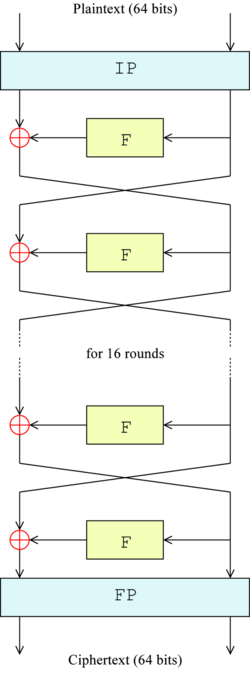
\includegraphics[scale=0.4]{DESwiki}
	\caption{Schéma du fonctionnement de DES avec les notations choisies (source : Wikipedia)}
	\label{deswiki}
\end{figure}


\begin{figure}[H]
\[
\begin{array}{|c|c|c|c|c|c|c|c|c|}
	\hline
	\text{Identifiant de la S-box $j$} & 1 & 2 & 3 & 4 & 5 & 6 & 7 & 8\\
	\hline
	\text{Niveau $i=1$} & 6 & 6 & 6 & 6 & 6 & 6 & 6 & 6\\
	\text{Niveau $i=2$} & 38 & 40 & 39 & 36 & 37 & 36 & 38 & 39\\
	\text{Niveau $i=3$} & 53 & 55 & 52 & 56 & 54 & 55 & 54 & 55\\
	\text{Niveau $i=4$} & 56 & 56 & 56 & 56 & 56 & 56 & 56 & 56\\
	\hline
\end{array}
\]
\caption{Nombre de bits de clé de dépendance pour chacun des bits en sortie des S-box à différents rounds. Le niveau correspond au
	nombre de rounds qu'on pourrait potentiellement gagner avec déchiffrement partiel.}
	\label{arraybit}
\end{figure}

\begin{figure}[H]
	\centering
	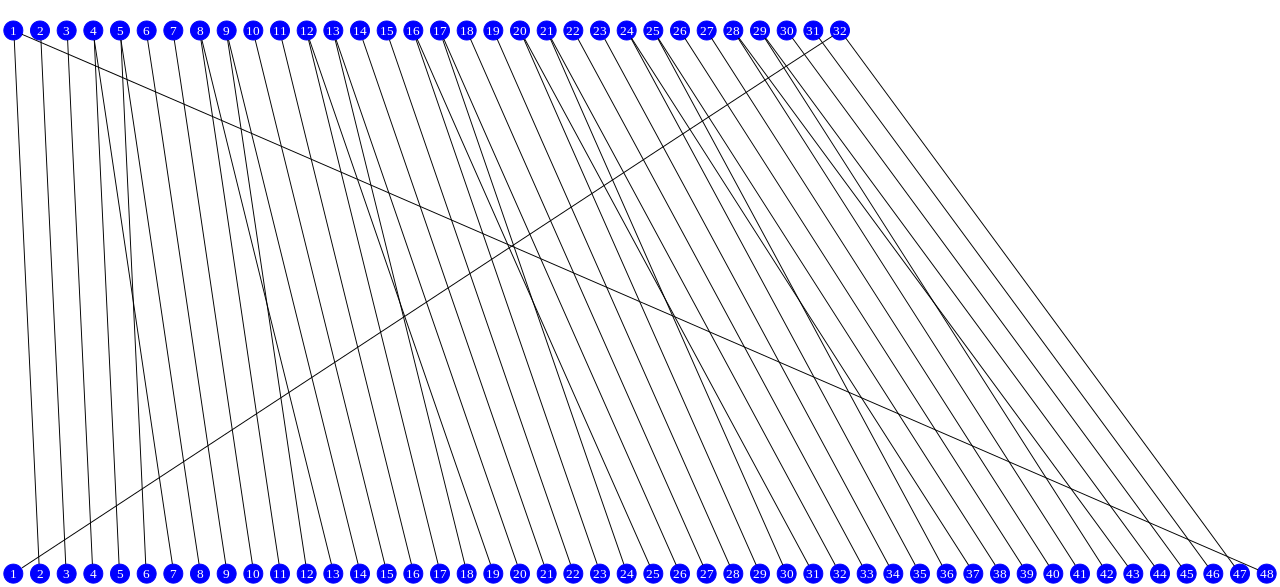
\includegraphics[scale=0.3]{exp}
	\caption{Schéma de la fonction d'expansion (source : Wikipedia)}
	\label{fig:exp}
\end{figure}

\begin{figure}
	\centering
	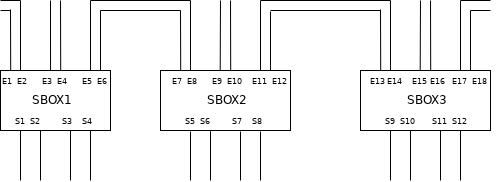
\includegraphics[scale=0.7]{schemainout}
	\caption{Schéma des entrées/sorties pour les trois premières S-box.}
	\label{fig:inout}
\end{figure}

\begin{figure}
	\centering
	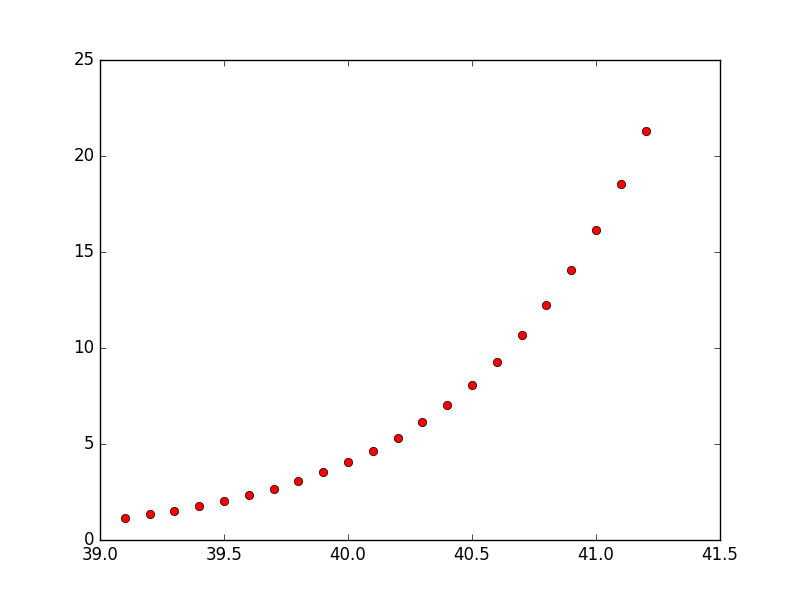
\includegraphics[scale=0.5]{fig1}
	\caption{Meilleur avantage théorique en fonction du logarithme de la complexité en donnée pour le DES sur 14 rounds. Tous les
	points correspondent en fait à la combinaison des deux listes d'approximations de Matsui.}
	\label{reftheo}
\end{figure}

\begin{figure}
	\[
		\begin{array}{|c|c|c|}
			\hline
			\text{Identifiant de l'approximation} & \text{Biais du premier ensemble} & \text{Biais du deuxième ensemble}\\
			\hline
			\text{Approximation 1} & 1.4648 \times 2^{-11} & 1.1250\times 2^{-12}\\
			\hline
			\text{Approximation 2} & 1.4648 \times 2^{-12} & 1.1250\times 2^{-13} \\
			\hline
			\text{Approximation 3} & 1.6875 \times 2^{-15} & 1.1250\times 2^{-13}\\
			\hline
		\end{array}
	\]
	\caption{Biais des approximations choisies}
	\label{bias}
\end{figure}



\begin{figure}
\[
	\begin{array}{|c|c|c|c|c|c|c|c|}
		\hline
		N & 2^{20} & 2^{22} & 2^{23} & 2^{24} & 2^{25} & 2^{25.5} & 2^{26}\\
		\hline
		R_{\text{min}} & 2^{54.205} & 2^{54.652} & 2^{40.340} & 2^{34} & 2^{41.175} & 2^{36} & 2^{32}\\
		\hline
		R_{\text{round}} & 2^{54.211} & 2^{54.658} & 2^{40.384} & 2^{34.322} & 2^{41.224} & 2^{36.170} & 2^{33}\\
		\hline
		R_{\text{max}} & 2^{54.211} & 2^{54.658} & 2^{40.384} & 2^{34.322} & 2^{41.224} & 2^{36.170} & 2^{33}\\
		\hline
		a_{\text{round}} & 1.789 & 1.342 & 15.616 & 21.618 & 14.776 & 19.830 & 23\\
		\hline
	\end{array}
\]
%2^23 
%min: 2^40.33985
%actual rounded: 2^40.38370429
%max: 2^40.38370429
%2^24
%min: 2^34
%actual rounded: 2^34.32192809
%max: 2^34.32192809
%2^25
%min: 2^41.17492568
%actual rounded: 2^41.22400167
%max: 2^41.22400167
%2^{25.5}
%min: 2^36
%actual rounded: 2^36.169925
%max: 2^36.169925
%2^26
%min: 2^32
%actual rounded: 2^33
%max: 2^33
%2^20
%min: 2^54.20506536
%actual rounded: 2^54.21089217
%max: 2^54.21089217
%2^22
%min: 2^54.65223732
%actual rounded: 2^54.65799503
%max: 2^54.65799503

	\caption{Résultats des simulations. $R_{\text{min}}$ est une borne inférieure du rang de la clé,
	obtenue avec l'algorithme de RE. De même, $R_{\text{round}}$ et $R_{\text{max}}$ représentent
	respectivement le rang espéré et une borne supérieure. $a_{\text{round}}$ est l'avantage correspondant
	à $R_{\text{round}}$.}
	\label{result}
\end{figure}



\end{document}
